\chapter{Implementation}
\label{chap:implementation}

Initially, the implementation was divided into two parts. We discuss the implementation of \glsxtrshort{raptor} for the browser in \autoref{section:implementation_raptor}. The conversion and download of GTFS data is discussed in \autoref{section:implementation_data_ontology}.


\section{\glsfmtfull{raptor} implementation}\label{section:implementation_raptor}
\subsection{Data usage of existing implementation}
Since an existing implementation of Raptor inspired us, we researched which data the implementation used.

Small description of the used text files in the \glsxtrshort{gtfs}-feed and how they are transformed.
\begin{itemize}
    \item \textbf{calendar.txt}: Used to create an Calendar Object with a "service\_id" as key
    \item \textbf{stops.txt}: to create a Stop object with key stop\_id
    \item \textbf{calendar\_dates.txt}: Creates a Dates object with key service id. Holds all key dates on which a service is active. Using exception\_type === "1" (service exceptions)
   \item \textbf{trips.txt}: Creates a huge array of trips.
   \item  \textbf{stop\_times.txt}: Used to create a list of Stoptimes with key trip\_id.
   
   \item \textbf{transfers.txt}: This creates two objects. If the transfer is from and to the same stop, we create an "interchange" object. But else we create a "transfers" object with a key "from\_stop\_id".
\end{itemize}

\subsubsection{Not used but are in our \glsxtrshort{gtfs}-feed}
\begin{itemize}
    \item feed\_info: Information of the feed itself. The publisher is not necessarily the agency itself.
    \item agency: Information about the agency providing the services.
    \item areas: Optional file, Defines area identifiers.
    \item translations: Optional file, useful for a country with multiple languages.
\end{itemize}
\subsubsection{Unavailable in feed}
There are a lot of files that are marked as optional in the reference \cite{noauthor_gtfs_2022} that are not present in our file:
fare\_attributes.txt,
    fare\_rules.txt,
    timeframes.txt,
    fare\_media.txt,
    fare\_products.txt,
    fare\_leg\_rules.txt,
    fare\_transfer\_rules.txt,
    stop\_areas.txt,
    networks.txt,
    route\_networks.txt,
    shapes.txt,
    frequencies.txt,
    pathways.txt,
    levels.txt,
    location\_groups.txt,
    location\_group\_stops.txt,
    locations.geojson,
    booking\_rules.txt and
    attributions.txt

\subsection{Small mistakes of the implementation}
\subsubsection{unused information from gtfsfeed}
The algorithm did not use some information but was thereby inferred. For example:
\begin{itemize}
    \item Order of stop points. Each stop point in a sequence was based on its position in the array, which is not a big problem if the array is correctly sorted. But a \glsxtrshort{gtfs} feed requires each stop point to carry information like their position in the sequence. This is more correct since it supports feeds with incorrectly sorted stop points.
    \item Route id was not used but created from the trip\_id and all the stop times in that trip. Since our solution will be more dynamic and not include all stop times simultaneously, we will not follow the same structure.
\end{itemize}
\subsection{Important classes}
The \glsxtrshort{raptor} implementation is modular and contains a few classes:
\begin{itemize}
    \item \textbf{RaptorAlgortihmFactory}: This is a factory to create a RaptorAlgorithm instance. Before creating such an instance, it indexes the data it gets from the \glsxtrshort{gtfs}-parser.
    \item \textbf{QueueFactory}: This creates a queue on each iteration of the \glsxtrshort{raptor} algorithm.
    \item \textbf{RouteScanner}: This returns the earliest trip of a route, remembers the last trip in reference, and will not return the trip twice. This is essentially an iterator over trips in a route.
    \item \textbf{raptorAlgorithm}:Implementation of the \glsxtrshort{raptor} algorithm
\end{itemize}
\subsection{DataLoader: a new class}
The old implementation used a data flow that was unhandy for our goal. First, the RaptorAlgorithmFactory received the data that was parsed by the old parser. It then proceeded to create indexes and data structures. Then, it spreads that data to the relevant classes to create a RaptorAlgorithm.

\makeatletter
\begin{figure}[H]
\centering
\resizebox{.8\textwidth}{!}{%
    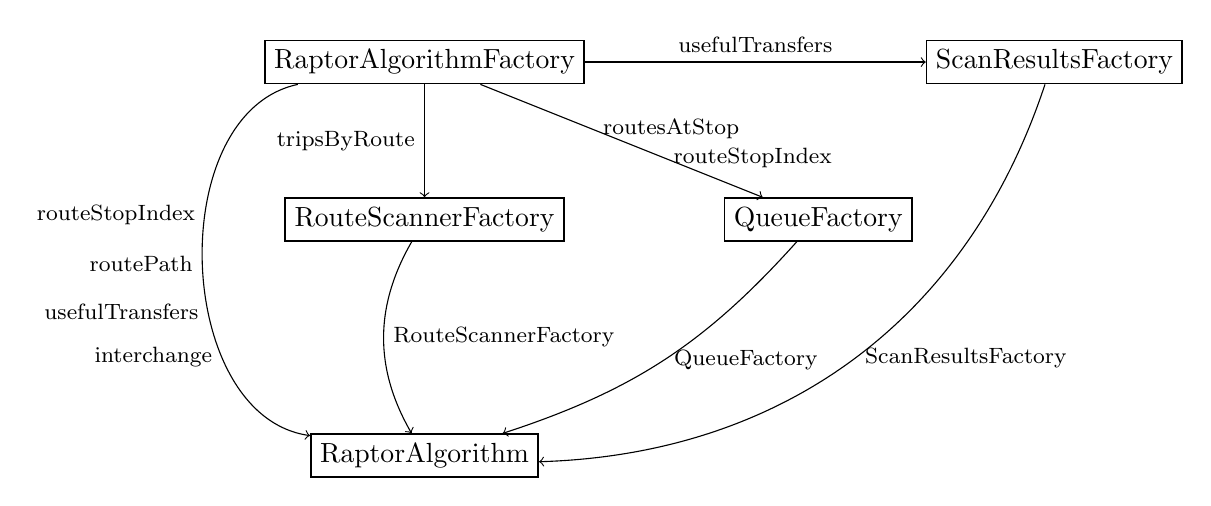
\begin{tikzpicture}[rect/.style={shape=rectangle,draw=black,semithick,align=center},
    ]
    % QueueFactory(, ),
    %       new RouteScannerFactory(tripsByRoute),

        
    % draw nodes
    \node[rect] (RaptorAlgorithmFactory) at (2,0) {RaptorAlgorithmFactory};
    \node[rect] (ScanResultsFactory) at (10,0) {ScanResultsFactory};
    \node[rect] (QueueFactory) at (7,-2) {QueueFactory};
    \node[rect] (RouteScannerFactory) at (2,-2) {RouteScannerFactory};

    \node[rect] (RaptorAlgorithm) at (2,-5) {RaptorAlgorithm};
    
    \draw (RaptorAlgorithmFactory) edge[->] node[above,pos=0.5,font=\footnotesize] {usefulTransfers} (ScanResultsFactory);

    \draw (RaptorAlgorithmFactory) edge[->] node[right,pos=0.4,font=\footnotesize] {routesAtStop} node[right,pos=0.65,font=\footnotesize] {routeStopIndex} (QueueFactory);

    \draw (RaptorAlgorithmFactory) edge[->] node[left,pos=0.5,font=\footnotesize] {tripsByRoute} (RouteScannerFactory);

    \draw (RaptorAlgorithmFactory) edge[->, bend right=80] node[left,pos=0.4,font=\footnotesize] {routeStopIndex} node[left,pos=0.5,font=\footnotesize] {routePath} node[left,pos=0.6,font=\footnotesize] {usefulTransfers} node[left,pos=0.7,font=\footnotesize] {interchange} (RaptorAlgorithm);
    
    \draw (RouteScannerFactory) edge[->,bend right=30] node[right,pos=0.5,font=\footnotesize] {RouteScannerFactory} (RaptorAlgorithm);

    \draw (QueueFactory) edge[->, bend left=15] node[right,pos=0.5,font=\footnotesize] {QueueFactory} (RaptorAlgorithm);

    \draw (ScanResultsFactory) edge[->,bend left=35] node[right,pos=0.5,font=\footnotesize] {ScanResultsFactory} (RaptorAlgorithm);
    
    \end{tikzpicture}
    }
    \caption{This represents the dataflow of the \glsxtrshort{raptor} in order to createan RaptorAlgorithm}
    \label{fig:dataflow}
\end{figure}
\makeatother

A new class, Dataloader, was created to hold all data in one class. Additionally, the class will also handle all requests for new fragments and process these new fragments to populate the needed data structures.

We did this by moving the following data holders to the DataLoader class and making them a private field. For each private field, a getter/setter is generated.
\begin{itemize}
    \item \textbf{tripsByRoute}: This holds all the trips corresponding to a route. Primarily used by RouteScanner, which uses this to give back an interesting trip for the \glsxtrshort{raptor} algorithm.
    \item \textbf{routeStopIndex}: Contains all the corresponding stops of a route; for each stop, it stores the index in the route.\\ For example $\{route\_id\_1:\{stop\_id\_1:1,stop\_id\_2:2\}\}$.
    \item \textbf{routePath}: Contains a list of stop IDs for each route.\\ For example: $\{route\_id\_1:[stop\_id\_1,stop\_id\_2]\}$
    \item \textbf{routesAtStop}: This contains a list of all possible routes (regardless of whether a trip is running or not) possible at a given stop.
    \item \textbf{interchange}: This list defines how long a transfer in the same station takes.
    \item \textbf{usefulTransfers}: A list of transfers between nearby stations. For example, stations 100 meters away can be done by foot.
\end{itemize}

We then changed RouteScanner, RouteScannerFactory, ScanResults, ScanResultsFactory and QueueFactory to use our new class.

To the constructor of the Dataloader, we also pass the origin and destination. Then, after creation, we call the function "first". This function gets the first fragment starting from the origin. Since we had to await the request for the fragment, we could not place this in the constructor since in \glsxtrshort{js}, constructors can not be made async.

\makeatletter
\begin{figure}[H]
\centering
\resizebox{.8\textwidth}{!}{%
    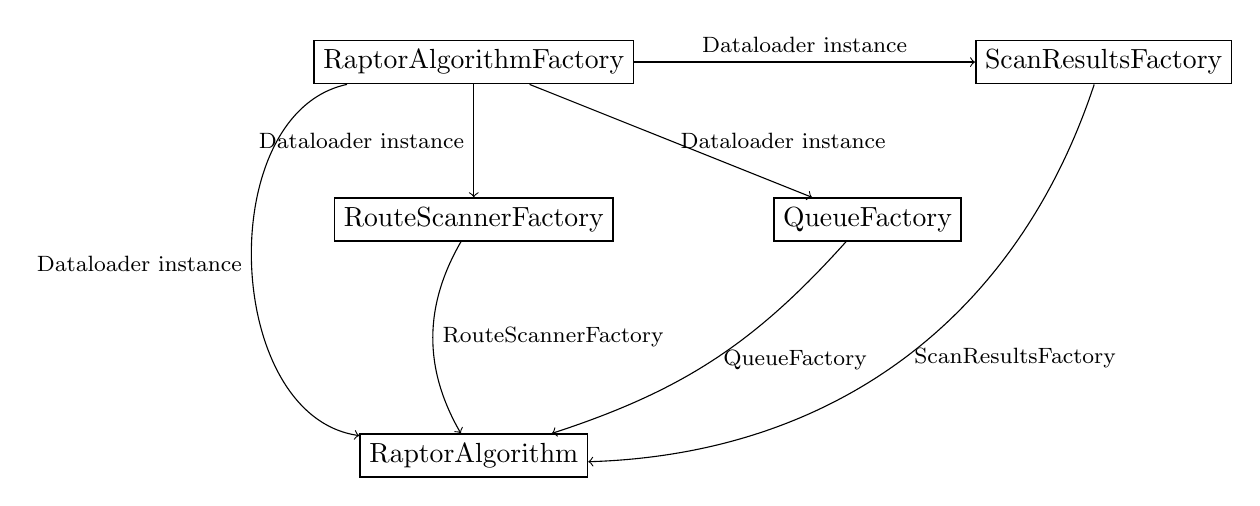
\begin{tikzpicture}[rect/.style={shape=rectangle,draw=black,semithick,align=center},
    ]

    % draw nodes
    \node[rect] (RaptorAlgorithmFactory) at (2,0) {RaptorAlgorithmFactory};
    \node[rect] (ScanResultsFactory) at (10,0) {ScanResultsFactory};
    \node[rect] (QueueFactory) at (7,-2) {QueueFactory};
    \node[rect] (RouteScannerFactory) at (2,-2) {RouteScannerFactory};

    \node[rect] (RaptorAlgorithm) at (2,-5) {RaptorAlgorithm};
    
    \draw (RaptorAlgorithmFactory) edge[->] node[above,pos=0.5,font=\footnotesize] {Dataloader instance} (ScanResultsFactory);

    \draw (RaptorAlgorithmFactory) edge[->] node[right,pos=0.5,font=\footnotesize] {Dataloader instance} (QueueFactory);

    \draw (RaptorAlgorithmFactory) edge[->] node[left,pos=0.5,font=\footnotesize] {Dataloader instance} (RouteScannerFactory);

    \draw (RaptorAlgorithmFactory) edge[->, bend right=80] node[left,pos=0.5,font=\footnotesize] {Dataloader instance} (RaptorAlgorithm);
    
    \draw (RouteScannerFactory) edge[->,bend right=30] node[right,pos=0.5,font=\footnotesize] {RouteScannerFactory} (RaptorAlgorithm);

    \draw (QueueFactory) edge[->, bend left=15] node[right,pos=0.5,font=\footnotesize] {QueueFactory} (RaptorAlgorithm);

    \draw (ScanResultsFactory) edge[->,bend left=35] node[right,pos=0.5,font=\footnotesize] {ScanResultsFactory} (RaptorAlgorithm);
    
    \end{tikzpicture}
    }
    \caption{This represents the new dataflow of the \glsxtrshort{raptor} to create a RaptorAlgorithm. Note that RaptorAlgorithmFactory first creates an instance of Dataloader and shares that instance.}
    \label{fig:dataflownew}
\end{figure}
\makeatother

\subsection{Adapt for the browser}
The browser can run compiled Typescript or JavaScript natively. Initially, these \glsxtrshort{js} applications were pretty small, but over recent years, they got bigger. This has been sped up by the introduction of Node.js, where \glsxtrshort{js} is used in a different context. 

This created a need for a way to split up \glsxtrshort{js}-applications into modules. Node.js already supports modules, but the good thing is that recently, the browser has also started to support modules. \cite{noauthor_javascript_2024}

This means we can easily import our \glsxtrshort{js} code after compiling the Typescript and then execute it in the browser.

To simplify the import, we bundle all our script files into one file using Esbuild \cite{noauthor_esbuild_nodate}. It is an extremely fast bundler that takes only 50 ms to bundle and transform our code. This is mainly because it is written in Go and compiles to native code. Further, it uses parallelisation and efficient use of memory.

Note this is even faster than the usual Typescript compile command $npm\ run\ tsc$!

Other handy options of the bundler are:
\begin{enumerate}
    \item \textbf{minify}: minify the code like whitespace. Reduces our code with 10 Kilobytes.
    \item \textbf{target}: Further optimisations can be unlocked with the option target. An example is \\$a === undefined || a == null? 1 : a$ could be minified to $a ?? 1$. Or, in reverse, transform \glsxtrshort{js} syntax that is too new for these environments into older JavaScript syntax that will work in these environments.
    \item \textbf{drop:console}: automatically remove all console statements.
    \item \textbf{sourcemaps}: This is essential for debugging. These maps encode the information necessary to translate from a line/column offset in a generated output file back to a line/column offset in the corresponding original input file. This is very handy if TypeScript or minification is used.
\end{enumerate}

The target option is essential because it ensures that all the node-specific APIs get converted to code supported by the browser.

\begin{listing}[H]
    \begin{minted}[frame=single,linenos, breaklines]{bash}
esbuild ./queries.js --bundle --sourcemap --target='chrome124,firefox124' --format=esm --outfile=browser.js
    \end{minted}
    \caption{Command to bundle our \glsxtrshort{js} code for debugging}
\end{listing}
\begin{listing}[H]
    \begin{minted}[frame=single,linenos, breaklines]{bash}
esbuild ./queries.js --bundle --target='chrome124,firefox124' --format=esm --outfile=browser.js --minify
    \end{minted}
    \caption{Command to bundle our \glsxtrshort{js} code for production}
\end{listing}
\section{GTFS downloader}
Since a GTFS feed is a zip file valid for a certain period, we need a small program to manage all these versions. This led to a Node.js module gtfs-downloader\footnote{Available as GitLab project under the same name. \\\url{https://gitlab.ilabt.imec.be/KNoWS/master-thesis/tibou-vanheule/gtfs-downloader}}. It provides the file path of the GTFS zip archive that either has been downloaded in the past or is freshly downloaded. So, it also acts like a cache and is more important than it appears, as only the most recent is available on the server. For debugging and experimenting while developing, it is handy that we have some control over the version in use. 

Two sets of functionality are represented in \autoref{fig:gtfsdownloader}. The first is when we already know the version we want to download. We search if it exists in our data folder; if not, we check if it is available on the server for download.

In the other case, we want to have the latest version, and we send a head request to the server\footnote{Server URL is specified in a dot env config} since we are only interested in the LastModified header. We check if that version is available locally; otherwise, we download the zip file.
\makeatletter
\begin{figure}[H]
\centering
\resizebox{.8\textwidth}{!}{%
    \begin{tikzpicture}[
        database/.style={
        path picture={
            \draw (0, 1.5*\database@segmentheight) circle [x radius=\database@radius,y radius=\database@aspectratio*\database@radius];
            \draw (-\database@radius, 0.5*\database@segmentheight) arc [start angle=180,end angle=360,x radius=\database@radius, y radius=\database@aspectratio*\database@radius];
            \draw (-\database@radius,-0.5*\database@segmentheight) arc [start angle=180,end angle=360,x radius=\database@radius, y radius=\database@aspectratio*\database@radius];
            \draw (-\database@radius,1.5*\database@segmentheight) -- ++(0,-3*\database@segmentheight) arc [start angle=180,end angle=360,x radius=\database@radius, y radius=\database@aspectratio*\database@radius] -- ++(0,3*\database@segmentheight);
        },
        minimum width=2*\database@radius + \pgflinewidth,
        minimum height=3*\database@segmentheight + 2*\database@aspectratio*\database@radius + \pgflinewidth,
    },
    database segment height/.store in=\database@segmentheight,
    database radius/.store in=\database@radius,
    database aspect ratio/.store in=\database@aspectratio,
    database segment height=0.1cm,
    database radius=0.25cm,
    database aspect ratio=0.35,
    roundnode/.style={circle, thick, minimum size=3em,align = center},
green/.style={draw=green!60, fill=green!5},
orange/.style={draw=orange!60, fill=orange!5},
white/.style={draw=black!60, fill=white},
    files/.style={double copy shadow,
        fill=white,
        draw=black,
        minimum width=5em,
        minimum height=2em}
    ]
        
    % draw nodes
    \node[files] (local) at (0,0) {local data};
    \node[roundnode,white] (program) at (8,0)  {GTFS downloader,\\ get specific version};
    \node[database, label=below:server gtfs.be] (server) at (15,0) {};

        % draw nodes
    \node[files] (local2) at (0,-5) {local data};
    \node[roundnode,white] (program2) at (8,-5)  {GTFS downloader,\\ get latest};
    \node[database, label=below:server gtfs.be] (server2) at (15,-5) {};
    % Draw edges
    \draw (local) edge[<-, bend left=15] node[pos=0.5,above] {1) check if local version exist} (program);
    \draw (local) edge[->,bend right=15] node[pos=0.5,below] {2) give filepath on existence} (program);
    \draw (program) edge[->,bend left=15] node[pos=0.5,above] {3) else check the server version} (server);
    \draw (program) edge[<-,bend right=15] node[pos=0.5,below] {4) Download file if  lastmodified and version match} (server);


    \draw (program2) edge[->, bend left=15] node[pos=0.5,above] {1) Head request} (server2);
    \draw (program2) edge[<-,bend right=15] node[pos=0.5,below] {2) headers of file: Lastmodified} (server2);
    \draw (program2) edge[->,bend right=15] node[pos=0.5,above] {3) check if latest version already exists} (local2);
    \draw (program2) edge[->,bend left=15] node[pos=0.5,below] {4) give filepath on existence} (local2);
    \draw (program2) edge[->,bend left=50] node[pos=0.5,above] {5) Download if not local} (server2);

    \end{tikzpicture}
    }
    \caption{Interaction model of the gtfs downloader.}
    \label{fig:gtfsdownloader}
\end{figure}
\makeatother
\section{Data parser/ontology}\label{section:implementation_data_ontology}
Since most datasets, including the datasets of the \glsxtrshort{nmbs} we use, use the \glsxtrshort{gtfs} Data model, we decided to write a program to convert \glsxtrshort{gtfs} to the \glsxtrshort{oslo} ontology.
\subsection{Ontology}
We decided to work with the \glsxtrshort{oslo} ontology. This is because they are based on a \glsxtrshort{epip} profile, which results in a less broad domain. Furthermore, since every European operator has to be compatible with Transmodel, this increases the usability of our research.

The ontology documentation includes data examples for "De Lijn", a Belgian bus operator. 

\subsubsection{Simplyfications}
The ontology is quite extensive and still has a large overview. The section of the overview we focus on has been included in the appendix \ref{appendix:oslo:ontology}. 

The ontology has some entities we do not need. For starters, we only have information about service journeys. Dead runs aren't included in our feed. Although \glsxtrshort{gtfs} can contain those trips, this is not the goal of \glsxtrshort{gtfs}. A specific field indicating whether a trip is a dead run is not in the reference \cite{noauthor_gtfs_2022}.

Entities representing dead runs are removed from our simplified overview. However, most service entities are specialisations, so we inherit the fields.

Additionally, we have no information about the shape of the routes. These shapes are used to view the route graphically in a routing app or on a map. The entities to define the order points in a route and the form of routes are neglected. We also edit the \glsxtrshort{shacl} file to change one cardinality constraint. 


We land on the following simplified overview:
\begin{figure}[H]
\resizebox{\textwidth}{!}{%
    \begin{tikzpicture}

\umlclass[x=0,y=0]{Line}{
  name : string \\ short\_name : string
}{}
\umlclass[x=6,y=0]{Route}{
  name : string
}{}

% connect line and route
\umlassoc[geometry=-|-, arg1=Line, mult1=0..1, pos1=0.3,  arg2=ConsistsOf, mult2=0..*, pos2=2, align2=left]{Line}{Route}

\umlclass[x=13,y=0]{Service Joruney pattern}{}{}
\umlassoc[geometry=-|-, arg1=Route, mult1=0..1, pos1=0.3, arg2=CoveredBy, mult2=0..*, pos2=1, align2=left]{Route}{Service Joruney pattern}
\umlclass[x=0,y=-6]{Planned Stop Point}{}{}
\umlclass[x=8,y=-3]{Passing Time}{}{}




%\umlnote[x=2.5,y=-6, width=3cm]{Route}{Je suis une note qui concerne la classe B}

    \end{tikzpicture}
    }
    \caption{Timeline describing the developments in route planning. The crossed parts represent}
    \label{fig:ontology}
\end{figure}

The classes have conceptually a lot in common with \glsxtrshort{netex} and Trnsmodel. 
\begin{itemize}
    \item \textbf{Line and route}: A representation of a line or route used to conceptualise a path in a network.
    \item \textbf{Service journey pattern}: Describes the order of points in a route. For each point in this class, a passenger can get off or on.
    \item \textbf{Stoppoint in service journey pattern}: Describes a visit of a service to a scheduled stop point. Give more information about if passengers can be dropped off or picked up.
    \item \textbf{Schedueled Stop Point}: Conceptualizes a point where passengers visit. It also links with a physical stop point, defined in another vocabulary.
    \item \textbf{Service journey}: is a vehicle journey allowing passengers to get on or off.
    \item \textbf{Passing time}: Describes the visit in time of the vehicle to a stopping point.
    \item \textbf{Service Calendar}: Describes on which days a trip is 
\end{itemize}

We will not include all the information in our fragment for the client because not everything is needed. We first fixate to supply the necessary data for route calculation. As a starting point, we take the scheduled Stop point entity. This provides all the passing times in a specific station and contains all service links. A service link is a service connection between two scheduled stop points. When such a connection exists, it means at least one trip exists, which a passenger can take to travel to a different station.

\begin{figure}[H]
\resizebox{\textwidth}{!}{%
    \begin{tikzpicture}[
rect/.style={shape=rectangle,draw=black,semithick,align=center},
green/.style={draw=green!60, fill=green!5},
orange/.style={draw=orange!60, fill=orange!5},
white/.style={draw=black!60, fill=white}    ]
        
    % draw nodes

    \node[rect] (passtime) at (5,-2)  {Passing Time};

    \node[rect] (servicelink) at (16,-4)  {Service Link};
    
    \node[rect] (stoppointinshedueled) at (10,-2)  {Stop point in Service pattern};

    \node[rect,draw=red] (schechedueledstoppoint) at (10,-4)  {scheduled Stop Point};

    \node[thick,text=red] (extra_info) at (10,-5)  {main entry};


    \draw (extra_info) edge[->,thick,color=red] (schechedueledstoppoint);


    % EDGE stoppoint in pattern and scheduled stop point
    \draw (stoppointinshedueled) -- node[pos=0.2,left, font=\footnotesize] {seen as} node[pos=0.2,right, font=\footnotesize] {0..*}  node[pos=0.8,left, font=\footnotesize] {View of} node[pos=0.8,right, font=\footnotesize] {1}
    (schechedueledstoppoint);

    % Passing time and stop point in rit pattern
    \draw (passtime) edge[-{diamond[]}] node[pos=0.7,above, font=\footnotesize] {At}
    node[pos=0.7,below, font=\footnotesize] {0..*} (stoppointinshedueled);

    % service link edges
    \draw (servicelink) -- node[pos=0.8,above, font=\footnotesize] {From, 1 } node[pos=0.3,above, font=\footnotesize] {Start Of, 0..* }
    node[pos=0.3,below, font=\footnotesize] {End Of, 0..* }
    node[pos=0.8,below, font=\footnotesize] {To, 1 } (schechedueledstoppoint);

    \end{tikzpicture}
    }
    \caption{Simplified overview of the \glsxtrshort{oslo} ontologycentered around a shedueled stop point.} 
    \label{fig:ontology:entry}
\end{figure}

\subsubsection{Problems with the \glsfmtshort{oslo} \glsfmtshort{jsonld} context}
When we first downloaded the ontology, we noticed it wouldn't work in the \glsxtrshort{jsonld} playground. Upon closer inspection, we noticed that the context contained empty types. We filled them in the blank and stored a corrected version in MongoDB. This is why, in all examples, the context points to \url{https://mx2.tibovanheule.space/ontology/context} instead of the context of \glsxtrshort{oslo}.
\begin{listing}[H]
    \begin{minted}[frame=single]{jsonld}
        @type: "";
    \end{minted}
    \caption{Problem with \glsxtrshort{oslo} context}
    \label{code:context:problem}
\end{listing}

\subsection{Parser}
The initial plan was to reuse the parser, but it used a package called gtfs-stream \cite{noauthor_staecogtfs-stream_2024}. The module takes a Readable stream object of a \glsxtrshort{gtfs} zip file and creates a pipe stream. The stream provides you  with an object with one of the following types: String, feed\_info, agency, stop, route, trip, stop\_time, calendar, calendar\_date, fare\_attribute, fare\_rule, shape, frequency, transfer)

This package is excellent if you want to read a \glsxtrshort{gtfs}-feed, but the package has one significant shortcoming for converting a feed to a different ontology. Defining the order in which the module reads the files is impossible. For example, this is not possible if you want to read about the trips before stop times.

We chose to implement something similar but without the gtfs-stream module. 
\subsubsection{Node streams}
First, we explain NodeJS streams. A stream is an abstract interface for working with streaming data in Node.js. \cite{noauthor_stream_nodate} They are similar to arrays and other collections. But what makes them powerful is that not all data is available, so they do not have to fit in memory all at once. Especially when working with big data sets.

They are either readable or writeable.

\subsubsection{our \glsfmtshort{gtfs} streamer}
To have more control over how to read files of a \glsxtrshort{gtfs} feed, we implemented our own \glsxtrshort{gtfs} streamer with two modules.



The first module is a zip reader called node-stream-zip \cite{noauthor_node-stream-zip_2021}. Like the \glsxtrshort{gtfs}-stream package, it creates a readable stream object and gives back a stream. A real improvement is that we can provide a filename that we want to extract from the zip file. It is unnecessary to read the full \glsxtrshort{gtfs} file. This offers excellent flexibility, solves the problem of ordering and gives immediate support for new files (if added in the \glsxtrshort{gtfs} specification) or out-of-spec files.

Now, we can read the files in the order we want and parse every line. Since \glsxtrshort{gtfs} is stored as \glsxtrshort{csv}, we can use any \glsxtrshort{csv} parser. We opted for csv-parse \cite{noauthor_csv-parse_2024}, a popular, well-known module. We give the parser the delimiter (",") and the columns option. The columns have the effect that the rows are returned as \glsxtrshort{json} objects instead of arrays.

\begin{listing}[H]
\inputminted[linenos,frame=single,breaklines]{TypeScript}{code/own_gtfs_streamer.js}
    \caption{Our own version of \glsfmtshort{gtfs}-streamer}
\label{listing:gtfs:streamer}
\end{listing}

\subsubsection{MongoDB}

\subsubsection{MongoDB: Bulk Write}
After reading the \glsxtrshort{csv} files correctly, we are left with converting the \glsxtrshort{json} object to the ontology and inserting them in MongoDB.

Some difficulties directly arose. We want to have a merged view in MongoDB. We did not want all entities in different collections. So, we had to insert the planned stop points and then update them when extra information became available. At first, we used the updateOne API from Mongodb. 
\begin{listing}[H]
    \begin{minted}[linenos,frame=single]{TypeScript}
let collection = connection.db(db_name).collection(collection_name);
return collection.updateOne(id, update);
    \end{minted}
    \caption{Usage of updateOne in mongoDB}
\label{listing:mongoDB:updateone}
\end{listing}
The problem with that is the combination of updateOne in a NodeJS stream. Quickly, the memory begins to rise, eventually crashing the program due to a lack of system resources. A recommended npm module to monitor RAM is Express-status-monitor \cite{noauthor_express-status-monitor_2022}.

To avoid memory problems, we let each transformation function for a row of \glsxtrshort{csv} return a MongoDB write operation. These write operations can be given to bulkWrite of MongoDB. 

There are six types Of write operations:
\begin{enumerate}
    \item UpdateOne
    \item UpdateMany
    \item InsertOne
    \item DeleteOne
    \item DeleteMany
    \item ReplaceOne
\end{enumerate}

We further leverage Typescript to define a generic class to ease the programming burden. 

\begin{listing}[H]
    \inputminted[linenos,frame=single,breaklines]{TypeScript}{code/type_write_op.ts}
    \caption{A generic class with a constructor can easily create write operations.}
\end{listing}

\begin{listing}[H]
    \inputminted[linenos,frame=single,breaklines]{TypeScript}{code/type_write_op_instan.ts}
    \caption{An example of a possible instantiation of a generic class.}
\end{listing}
\subsubsection{MongoDB: Unordered execution}
Another important side note is that bulkWrite inserts are ordered. This means that bulkWrite executes the write operations in the same order as the array's order. This is not a huge problem, but some optimisation can be unlocked if we tell bulkWrite that the write operations may be executed unordered. This is primarily because the command can make better batch sizes. 

Another side effect of unordered execution is that if a duplicate key occurs or there are write operation errors, the other write operations are still executed. 

This difference in execution is because if we insert ordered, MongoDB assumes there is a dependence and the order of the operations matters. Hence, it won't continue if it encounters an error.

We execute Mongodb queries unordered since the order does not matter.

\section{Bringing two worlds together: Fragmenting}
\subsection{MongoDB: geospatial}
One way to start fragmenting is by leveraging the MongoDB spatial capabilities \cite{noauthor_geospatial_nodate}. MongoDB supports a few geospatial operations, such as near and within. For each of these operations, we also have the variant for the sphere. So, in general, it's not as powerful as Geopandas or PCraster. 

There are other downsides as well. MongoDB requires you to work with \glsxtrshort{geojson}, a format we do not use in our ontology. Our coordinates are saved as WKT literals. We must store the coordinates as \glsxtrshort{geojson} and WKT. WKT since we still conform to the application profile and \glsxtrshort{geojson} to enable the geospatial querying. Using projection in the queries, the server never returns the \glsxtrshort{geojson} data. 

Another downside is that Mongo requires creating a new index on the field containing the \glsxtrshort{geojson}. An index always comes with higher storage use and slows down inserts. Luckily, this is very manageable.

\subsubsection{\glsfmtfull{geojson}}
\glsxtrfull{geojson} \cite{butler_geojson_2016} is an open standard based on \glsxtrshort{json}. An Internet working group of \glsxtrshort{ietf} develops it. Which is uncommon compared to other GIS standards. 

It is meant to represent simple geographical features and their non-spatial attributes. 

\subsection{Near}
The first strategy involves selecting all Scheduled stop points within a certain distance of the source point. This is accomplished using the $\$near$ operator\cite{noauthor_near_nodate} from MongoDB. Since we use \glsxtrshort{geojson} data, we have to use the 2dsphere index. 

Further, we specify two options for the $\$near$ operator $\$maxDistance$ and $\$minDistance$.\\ $\$minDistance$ is of course set to zero and we let $\$maxDistance$ vary. 

Lastly, to create \glsxtrshort{geojson} as input for our search query, we first retrieve the corresponding document to our station node, then pass his coordinates to the $\$geometry$ operator.

\begin{listing}[H]
    \inputminted[linenos,frame=single,breaklines]{TypeScript}{code/near.ts}
    \caption{Implementation of the "near" fragment strategy using the $\$near$ operator.}
\end{listing}

An immediate drawback of this strategy is that we do not test the reachability of a scheduled stop point to the source node.

Not to mention, once we request a point that is outside our fragment, we will again apply the near strategy. This new fragment will overlap with the previous fragment. This is far from ideal.



However, the query returns quickly because we created a "2dsphere" index. We still notice that the response time is correlated to the distance we chose. 

\begin{figure}[H]
    \centering
    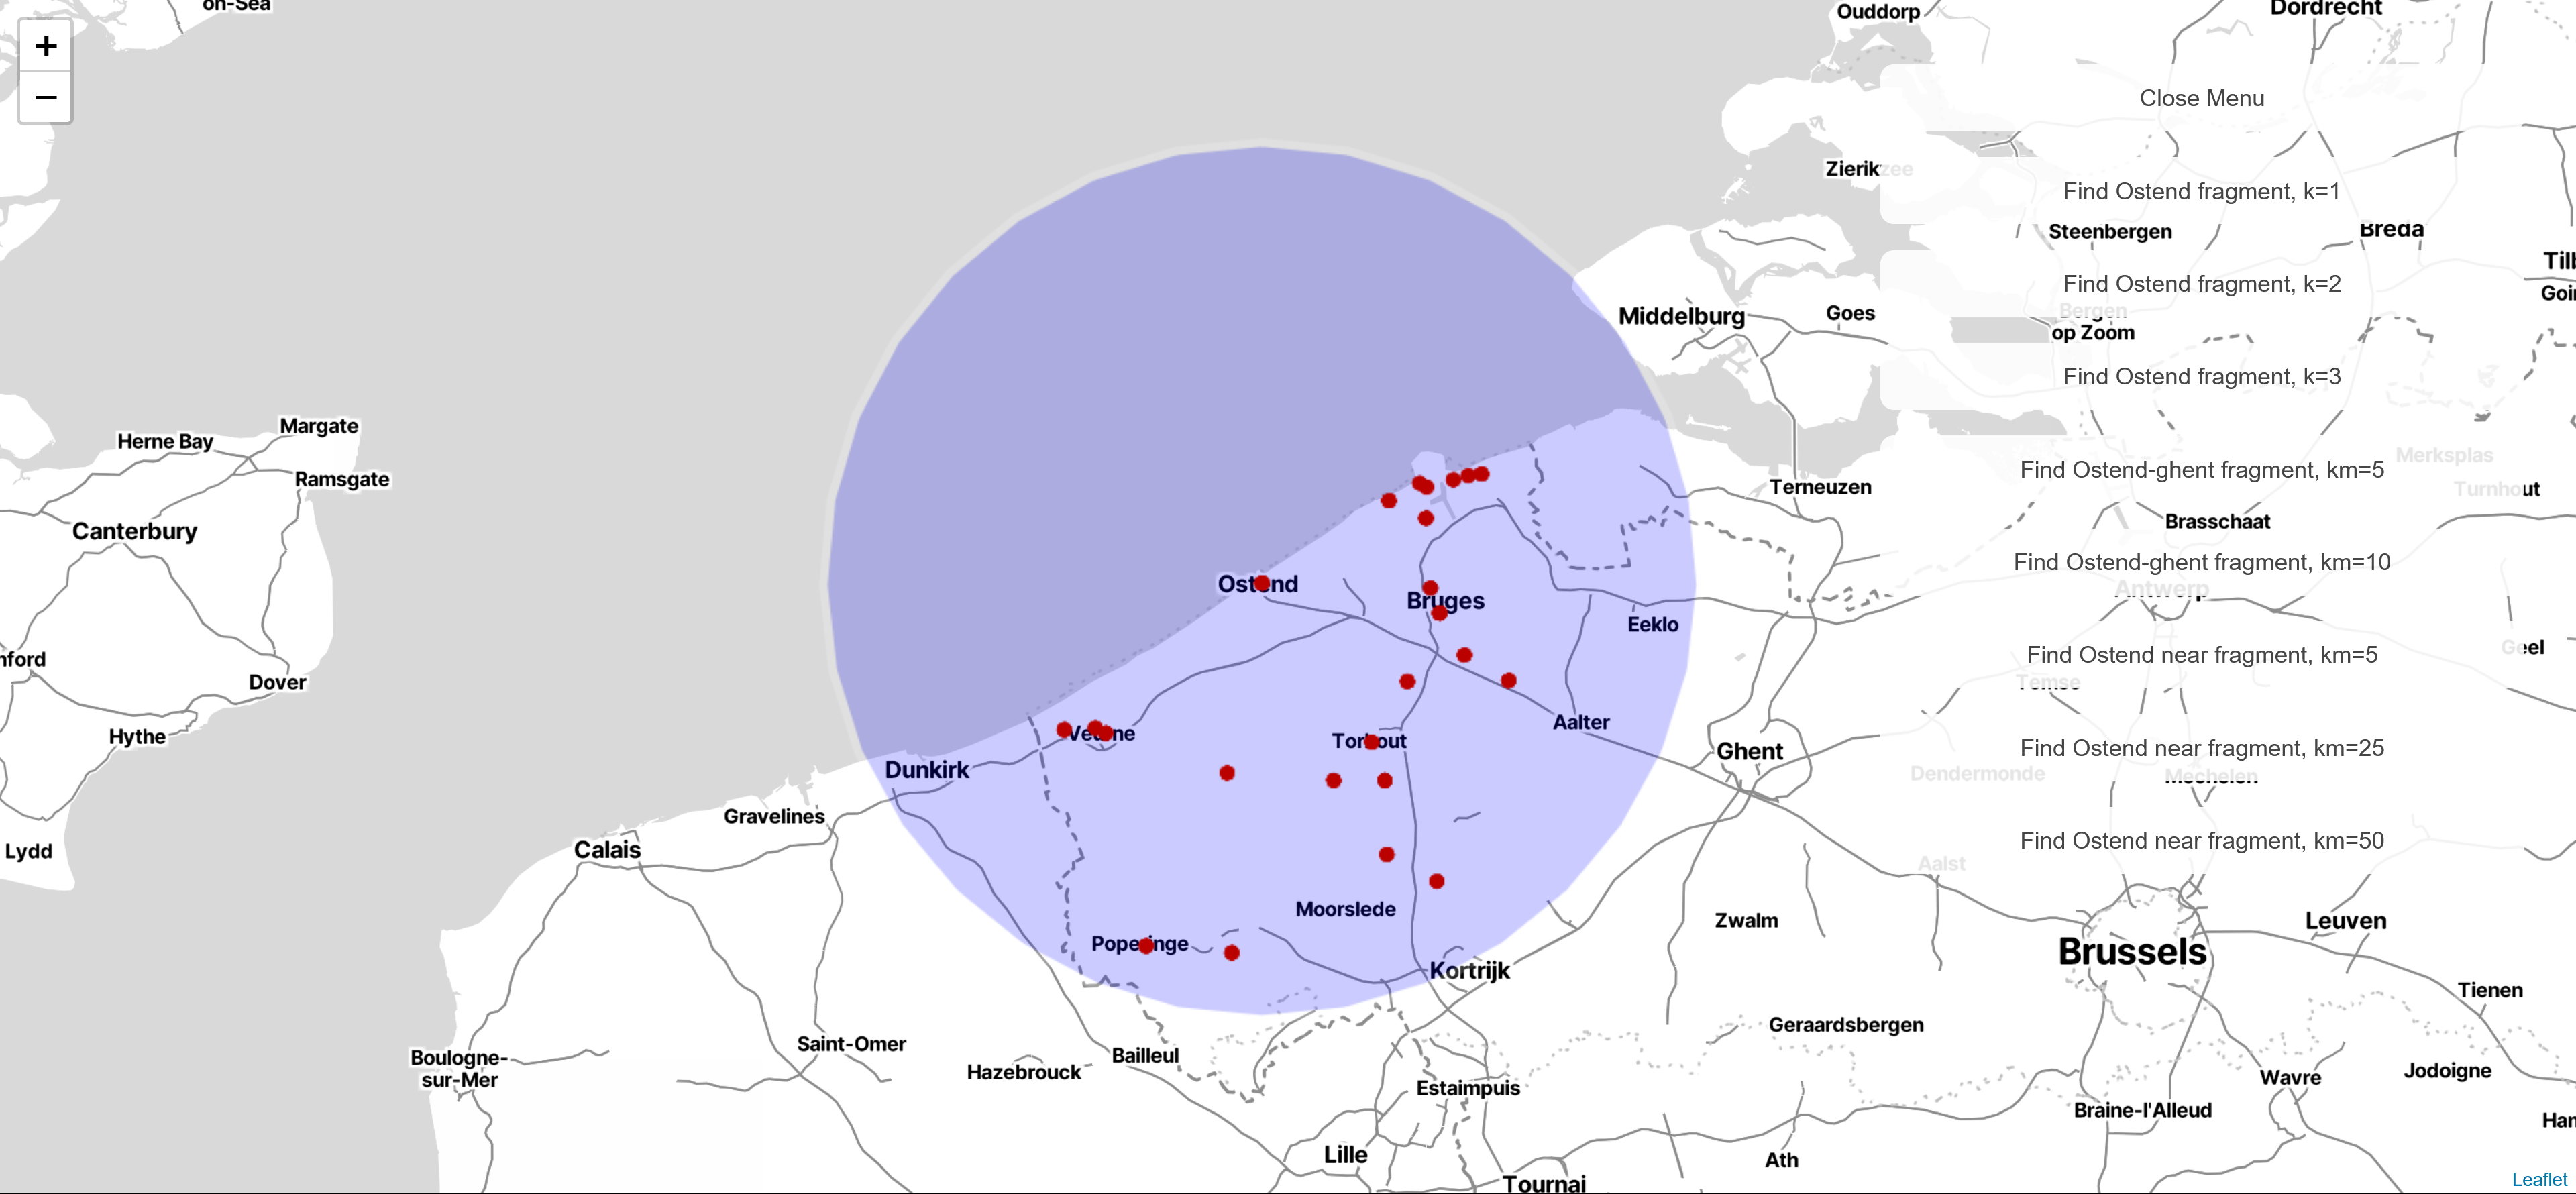
\includegraphics[width=\textwidth]{images/near visualized.png}
    \caption{Visualisation of the near fragment around Ostend with a radius of 50KM}
    \label{fig:near-visualized}
\end{figure}
\subsection{Within}
A second strategy is to work with both our source and target stations. Since we have both coordinates, we can easily create a Linestring. That is an \glsxtrshort{geojson} structure that represents a line on a map. We buffer that string to create a Polygon and select every scheduled stop point in this shape.

We use the $\$within$ \cite{noauthor_geowithin_nodate} operator of MongoDB. Like the $\$near$, we must create a special geospatial index, which requires \glsxtrshort{geojson} data.

This strategy suffers from drawbacks similar to those of near-strategy. It requires \glsxtrshort{geojson} data and a 2dsphere index. Of course, we still do not test if a scheduled stop point is reachable. So, the result could contain stop points that should not be sent to the client. 

However, compared with the near strategy. It could be that all necessary scheduled stop points are in the Polygon/fragment. This will probably depend on the hierarchy. The fragment often has many or all needed stops for long-distance train travel in a more local, e.g. city, bus network. This could quickly fall short. An example is when a bus drives in a loop, and the source and target station are far apart. This can be mitigated by choosing an appropriate buffer size or adapting one.

\begin{figure}[H]
    \centering
    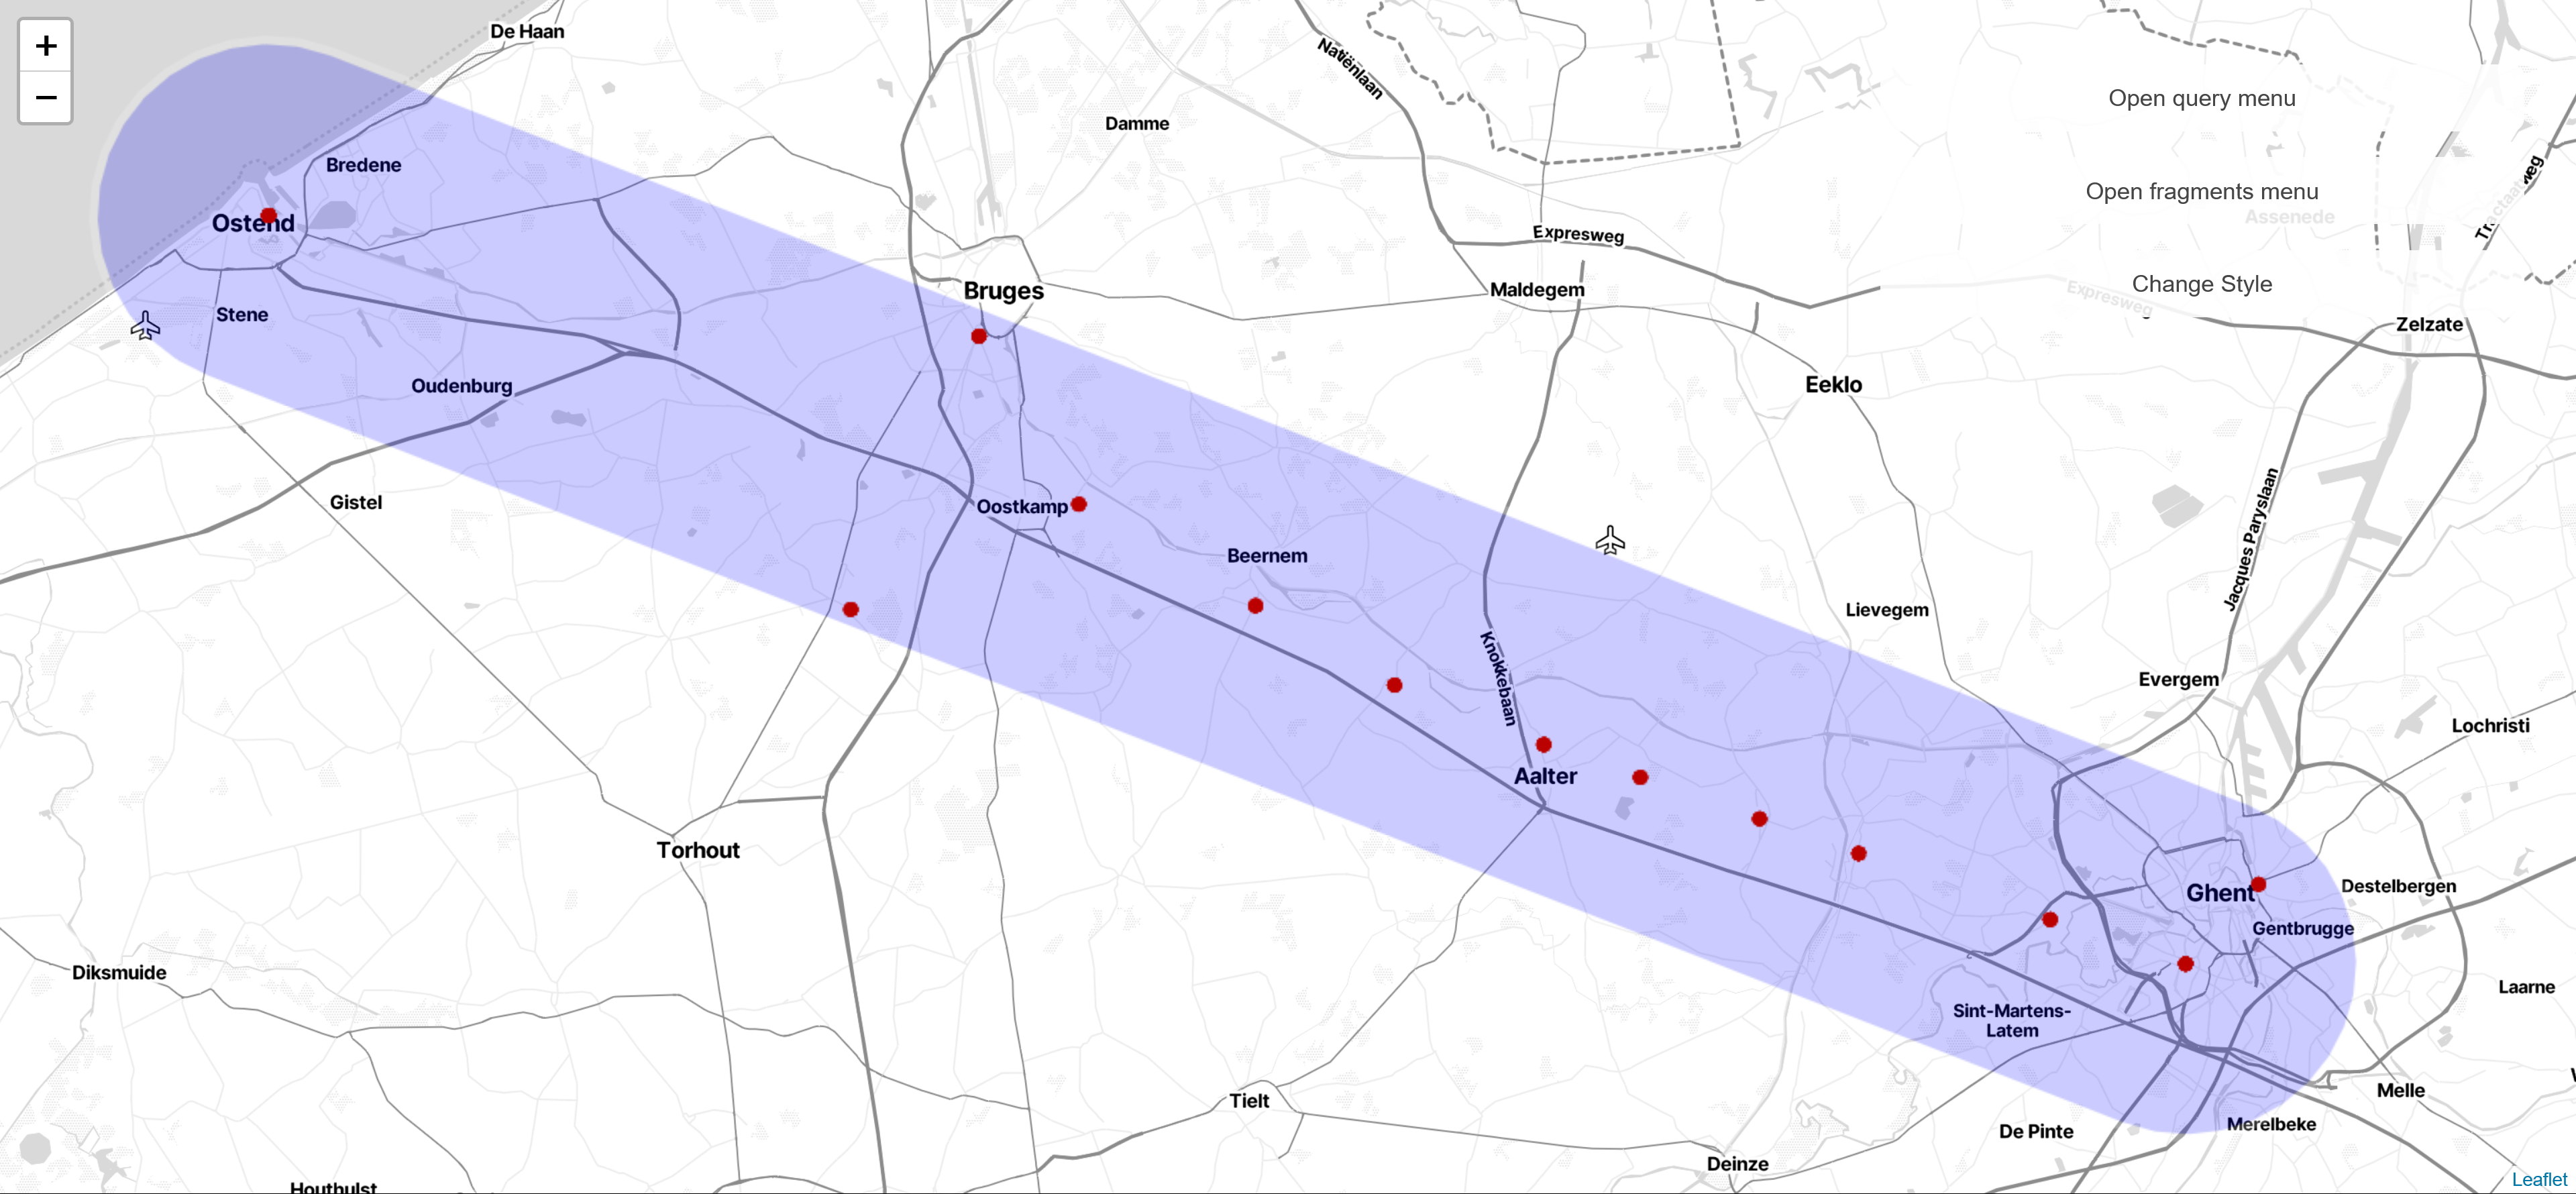
\includegraphics[width=\textwidth]{images/within visualized.png}
    \caption{Visualisation of the within fragment between Ostend and Ghent with a radius of 5KM}
    \label{fig:within-visualized}
\end{figure}

\subsubsection{Implementation}
We begin with retrieving the documents for both the source and target nodes. These coordinates in an array create a line string that we buffer. Since MongoDB does not support this kind of geo-operations, we use Turf\cite{noauthor_turfjs_nodate}.

\begin{listing}[H]
    \inputminted[linenos,frame=single,breaklines]{TypeScript}{code/turf.ts}
    \caption{Implementation of buffer lineString using the Turf library.}
\end{listing}

This buffer provides new coordinates that form a new Polygon. We can now use that polygon to test if a scheduled stop point lies in an area that is between our source and the target node.

\begin{listing}[H]
    \inputminted[linenos,frame=single,breaklines]{TypeScript}{code/within.ts}
    \caption{Implementation of the "within" fragment strategy using the $\$within$ operator.}
\end{listing}

\subsection{Reachable neighbours}
This strategy does not use MongoDB geospatial queries, so no index or geodata are needed. \\We use the $\$graphLookup$ \cite{noauthor_graphlookup_nodate} operator of MongoDB. The operator performs a recursive search. The API also allows the depth to be restricted or a branch to be stopped early when a given condition is met. 

It works by following these steps;
\begin{itemize}
    \item Takes documents as input, the start of aggregation pipeline.
    \item Targets the search to the collection designated by the from parameter.
    \item The search begins for each input document. The value of the field defined by startWith is used for the search.
    \item It matches the field value designated by connectToField in other documents in the "from" collection.
    \item For each matched document, it adds it to an array in the original document. 
    \item This recursively continues until no document is matched or the maximum depth is reached.
    \item Return results
\end{itemize}

In this approach, it is clear we immediately test whether another scheduled stop point is reachable. We consider only trips that leave a given station and arrive at another station.

\begin{figure}[H]
    \centering
    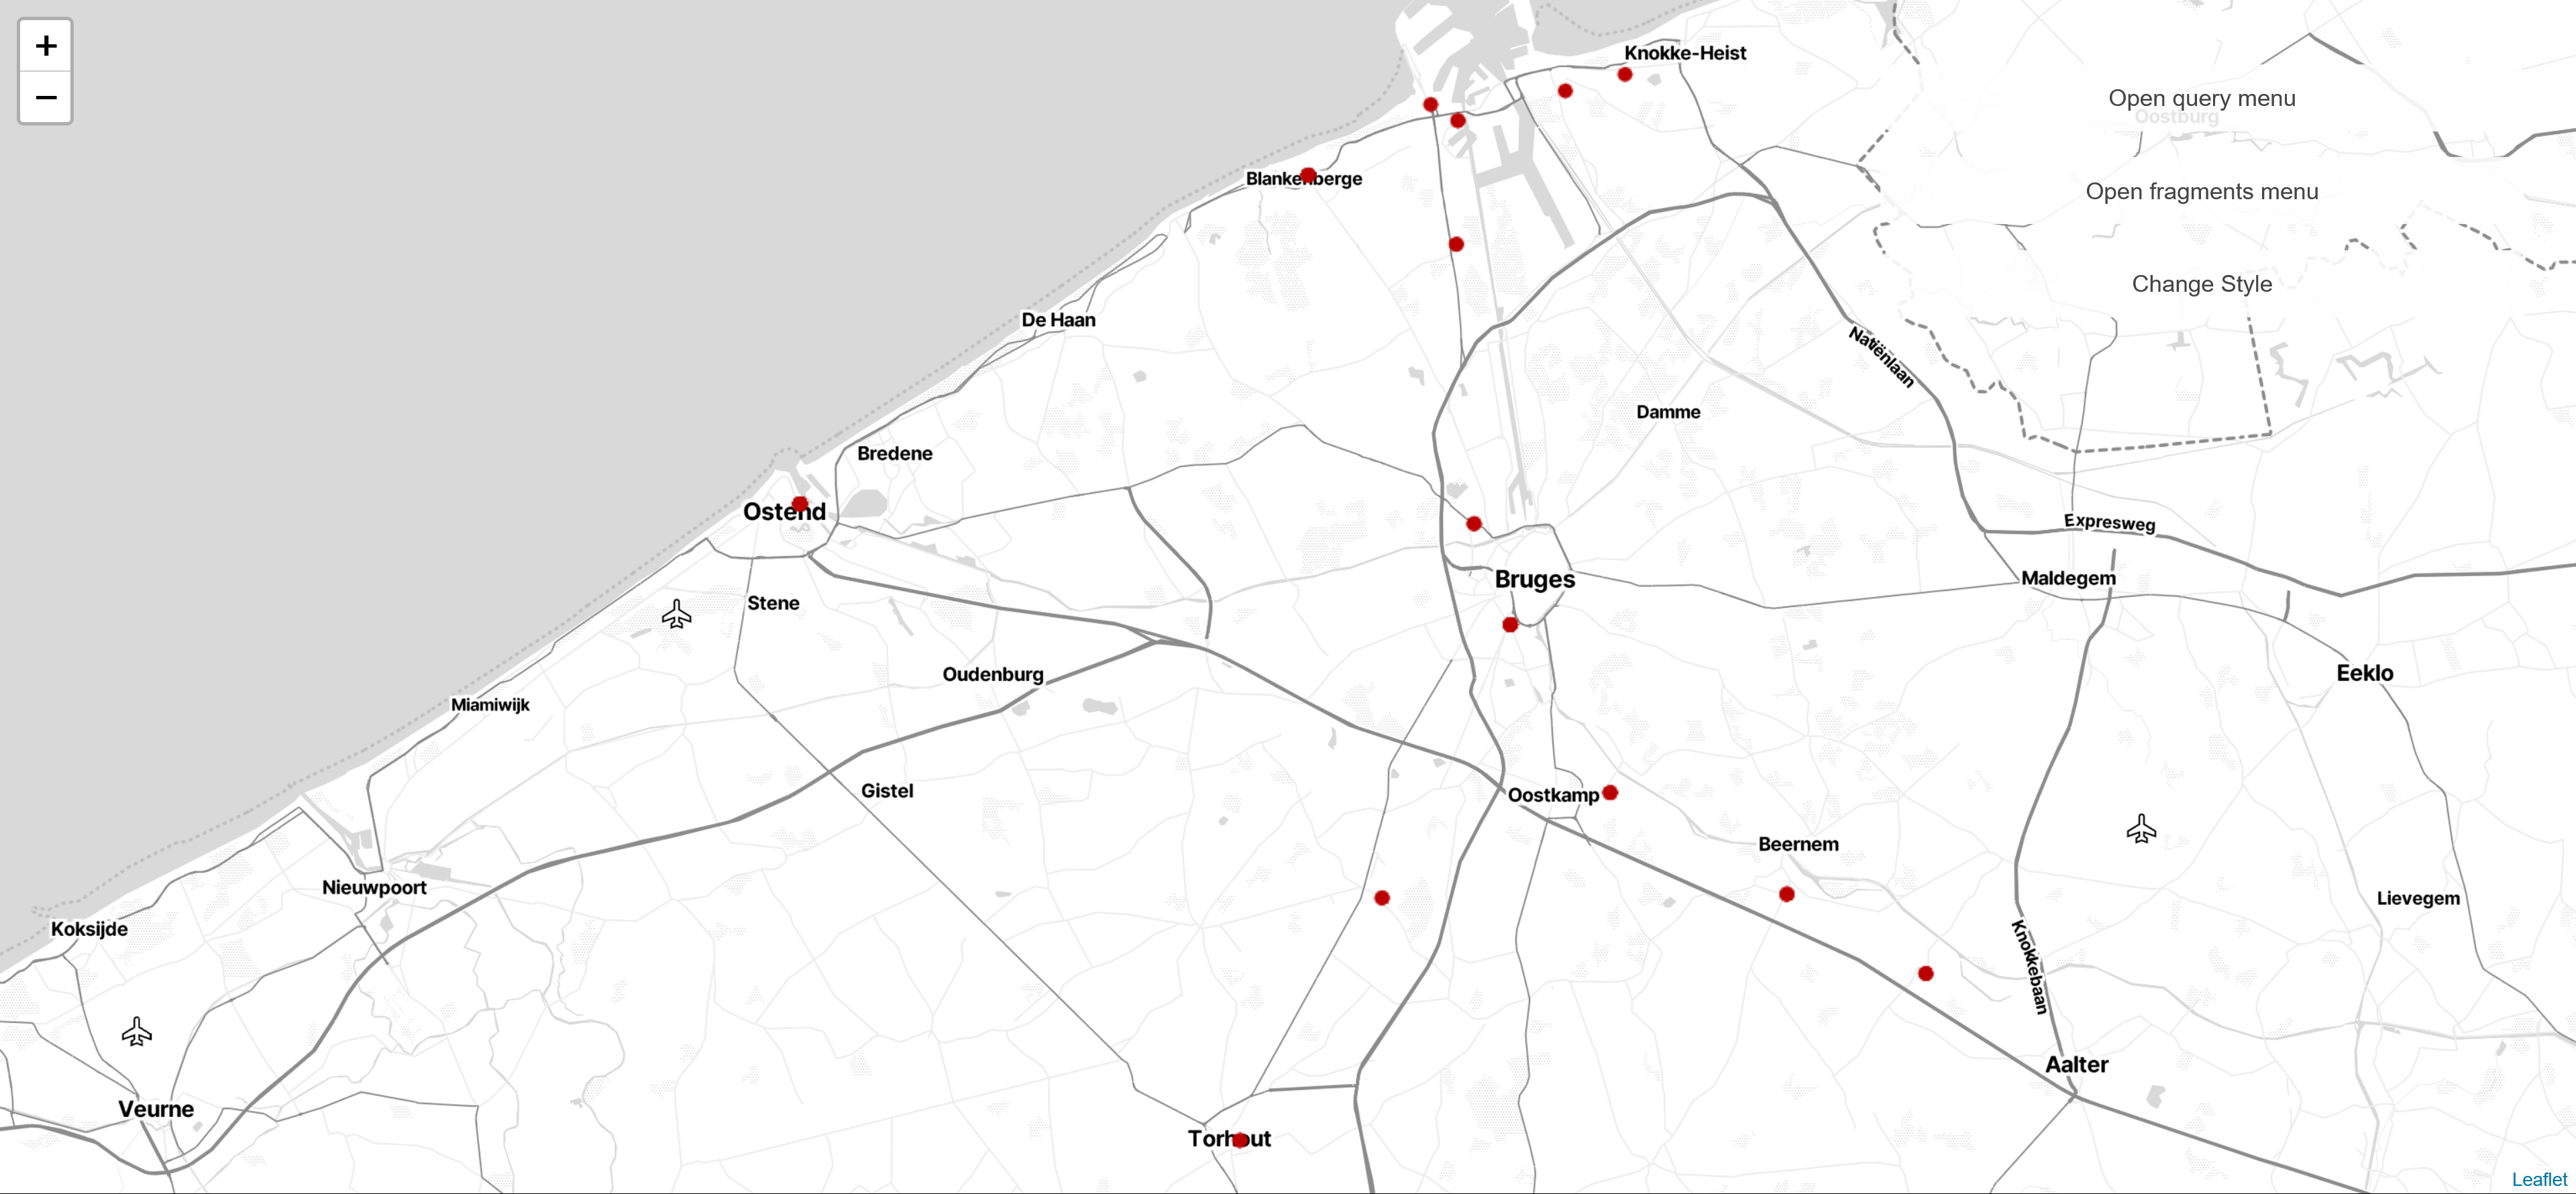
\includegraphics[width=\textwidth]{images/reacable visualized.png}
    \caption{Visualisation of the reachable fragment from Ostend with a depth of two}
    \label{fig:reachable-visualized}
\end{figure}

\subsubsection{Implementation}
Implementation is done in an aggregation pipeline, which results in a slightly more complicated pipeline. But we do not need to retrieve any document in a separate query. 

\begin{listing}[H]
    \inputminted[linenos,frame=single,breaklines]{TypeScript}{code/reachable.ts}
    \caption{Implementation of the "reachable neighbours" fragment strategy using the \\$\$graphLookup$ operator.}
\end{listing}

After that, we get one document with a field "neighbours." This array holds every connected scheduled stop point until depth k is reached. 

To convert this to one array, we run the following small code. 
\begin{listing}[H]
    \begin{minted}[linenos,frame=single,breaklines]{TypeScript}
        let list: any[] = [...t.neighbours]
        delete t["neighbours"]
        list.push(t)
    \end{minted}
    \caption{Post-processing of the $\$graphLookup$}
\end{listing}

This post-processing comes with a minor latency penalty.

\subsubsection{Implementation 2}
The first implementation has one big drawback. Mainly, MongoDB has a \glsxtrfull{BSON} limit of 16 megabytes for each document. Since graph lookup puts each neighbour in an array, this creates enormous problems. The Brussels station has many connections, so Graphlookup tries to place each document into the array. But on average, a Scheduled stop point with his passing times is around 300Kb in our dataset (\autoref{tab:mongodbstatres}). This means it quickly reaches the 16 MegaByte limit. 

We can implement the "graphlookup" pipeline using TypeScript and a for loop to avoid that. 

\begin{listing}[H]
    \inputminted[linenos,frame=single,breaklines]{TypeScript}{code/one_lookup_pipeline.ts}
    \caption{The output of this function is equal to graph lookup with depth = 0}
    \label{code:reachablejsimplementation}
\end{listing}


\subsection{Precomputed reachable neighbours}
Using the second implementation, we could precompute the reachable fragmentation strategy to speed up response times. To accomplish this, we changed \autoref{code:reachablejsimplementation}. After each loop iteration, we have a list of reachable neighbours with a k depth. We insert that list into a document. 

\begin{listing}[H]
    \begin{minted}[frame=single,linenos,breaklines]{JSON}
{
  "_id": "http://localhost:4600/1710486358000/GeplandStopPunt/8400530/k0",
  "neighbours": [
    "http://localhost:4600/1710486358000/GeplandStopPunt/8400530",
    "http://localhost:4600/1710486358000/GeplandStopPunt/8821105",
    "http://localhost:4600/1710486358000/GeplandStopPunt/8400131",
    "http://localhost:4600/1710486358000/GeplandStopPunt/8400526",
    "http://localhost:4600/1710486358000/GeplandStopPunt/8400561",
    "http://localhost:4600/1710486358000/GeplandStopPunt/8400058"
  ]
}
    \end{minted}
\end{listing}

When we want to retrieve all neighbours of a Stop point, we append the desired k-depth to the ID. We then retrieve the list and return all neighbours using find.

This last step comes with a little more complexity. We can use the $\$in$- operator of MongoDB to check if the $\_id$ is in a given array of values and, if so, return the found document. But this operator comes with a downside: it can not use indexes. A workaround combines the $\$or$ and $\$eq$ operators.
\begin{listing}[H]
\begin{minted}[linenos,breaklines,frame=single]{TypeScript}
return collection.find({
        $or: neighbours.map((el) => {
            return {_id: {$eq: el}}
        })
    }, {projection: {gepjson: 0}}).toArray();
\end{minted}
\caption{Retrieval of the precomputed neighbours.}
\end{listing}
\subsection{Overview}
\begin{table}[H]
\centering
\begin{tabular}{|l|l|l|l|l|l|}
\hline
\textbf{} &
  \textbf{near} &
  \textbf{withIn} &
  \textbf{\begin{tabular}[c]{@{}l@{}}reachable \\ neighbours\end{tabular}} &
  \textbf{\begin{tabular}[c]{@{}l@{}}precomputed \\ reachable neighbours\end{tabular}} &
  \textbf{\begin{tabular}[c]{@{}l@{}}precomputed \\ reachable neighbours \\and whitin\end{tabular}} \\ \hline
\textbf{GeoJSON required} & \cellcolor[HTML]{FD6864}yes & \cellcolor[HTML]{FD6864}yes & \cellcolor[HTML]{67FD9A}no  & \cellcolor[HTML]{67FD9A}no & \cellcolor[HTML]{67FD9A}no \\ \hline
\textbf{New index needed} & \cellcolor[HTML]{FD6864}yes & \cellcolor[HTML]{FD6864}yes & \cellcolor[HTML]{67FD9A}no  & \cellcolor[HTML]{67FD9A}no & \cellcolor[HTML]{67FD9A}no  \\ \hline
\textbf{\begin{tabular}[c]{@{}l@{}}Fragment can contain\\ unreachable stations\end{tabular}} &
  \cellcolor[HTML]{FD6864}yes &
  \cellcolor[HTML]{FD6864}yes &
  \cellcolor[HTML]{67FD9A}no &
  \cellcolor[HTML]{67FD9A}no &
  \cellcolor[HTML]{67FD9A}no \\ \hline
\textbf{independant of MongoDB api}      & \cellcolor[HTML]{FD6864}no & \cellcolor[HTML]{FD6864}no & \cellcolor[HTML]{FD6864}no  & \cellcolor[HTML]{67FD9A}yes& \cellcolor[HTML]{FD6864}no \\ \hline
\textbf{Can be calculated at runtime}          & \cellcolor[HTML]{67FD9A}yes & \cellcolor[HTML]{67FD9A}yes & \cellcolor[HTML]{67FD9A}yes & \cellcolor[HTML]{FD6864}no & \cellcolor[HTML]{FD6864}no  \\ \hline
\end{tabular}
\caption{Overview of fragment strategies.}
\label{tab:strategies}
\end{table}
To sum up our fragmentation story, we see that no real low-latency solution allows runtime computation. 
\subsubsection{Compression}
It immediately became clear that there are many Scheduled Stop Points because stations have multiple platforms. This quickly adds to many bytes, as seen in \autoref{fig:fragsize}. Even if we chose a low depth for the reachable neighbours strategy.

One way to mitigate this is to enable compression express middleware\cite{noauthor_compression_2019}. Using the default options, it will compress the response before sending if the threshold of 1Kb has been reached. When the client receives the data, it will uncompressed. 

Compression and decompressing have negative effects on response time. But for large transfers, it will greatly reduce the transfer size and time. 

\section{Demo}
Since the \glsxtrshort{raptor} has been browserified to run in the browser, it is pretty quick to develop a demo web app.

For this, we use some libraries and services:
\begin{itemize}
    \item \textbf{Leaflet} \cite{noauthor_leaflet_nodate}: It is an open-source library to create mobile-friendly interactive maps. It is used to overlay our results onto an OpenStreetMap map. 
    \item \textbf{GeoJSON-vt} \cite{noauthor_mapboxgeojson-vt_2024}: 
    \item \textbf{Leaflet-Geojson-vt} \cite{kshetri_iamteksonleaflet-geojson-vt_2024}: a plugin for Leaflet to use GeoJSON-vt.
    \item \textbf{Turf.js} \cite{noauthor_turfjs_nodate}: to add visualisations for the fragments strategies.
\end{itemize}

An online demo has been placed on \url{https://mx2.tibovanheule.space/raptor/}\footnote{This is not my fastest server}.
